\documentclass[sigplan,10pt]{acmart}

\usepackage[T1]{fontenc}
\usepackage[utf8]{inputenc}

\usepackage{acronym} % \ac[p], \acl[p], \acs[p], \acf[p]
\usepackage{algorithm} % \begin{algorithm} \end{algorithm}
\usepackage{algpseudocode} % \begin{algorithmic} \end{algorithmic}
\usepackage[inline]{enumitem} % \begin{enumerate*} \end{enumerate*}
\usepackage{tikz} % \begin{tikzpicture} \end{tikzpicture}

\usepackage{graphicx}
\usepackage{color}
\AtBeginDocument{
\definecolor{pdfurlcolor}{rgb}{0,0,0}
\definecolor{pdfcitecolor}{rgb}{0,0,0}
\definecolor{pdflinkcolor}{rgb}{0,0,0}
\definecolor{light}{gray}{.85}
\definecolor{vlight}{gray}{.95}
\definecolor{darkgreen}{rgb}{0.0, 0.2, 0.13}
\definecolor{mydarkblue}{RGB}{116,173,209}
\definecolor{mylightblue}{RGB}{171,217,233}
\definecolor{mydarkorange}{RGB}{244,109,67}
\definecolor{mylightorange}{RGB}{253,174,97}
\definecolor{mydarkred}{RGB}{215,48,39}
}

\usepackage[draft,inline,nomargin,index]{fixme}
\fxsetup{theme=colorsig,mode=multiuser,inlineface=\itshape,envface=\itshape}
\FXRegisterAuthor{go}{ago}{Gerald}
\FXRegisterAuthor{mn}{amn}{Matthieu}

\usepackage{subcaption} % subfigure

% Commands
%---------
\newcommand{\ie}{i.e. }

\newcommand{\inbb}[1]{\in \mathbb{#1}}
\newcommand{\mathlist}[2]{\set{#1_i \in #2}_{i \inbb{N}}}
\newcommand{\trm}[1]{\mathit{#1}}
\newcommand{\set}[1]{\left\{#1\right\}} % set brace notation

\newcommand{\id}[3]{$\trm{#1}^{\trm{#2}}_{\trm{#3}}$}

\newcommand{\widthletter}{7mm}
\newcommand{\widthblock}{11mm}

% Tikz styles
\tikzset{
    common/.style={anchor=west, draw, rectangle, minimum height=6mm},
    letter/.style={common, minimum width=\widthletter},
    block/.style={common, minimum width=\widthblock},
    cross/.style={
        path picture={
            \draw[mydarkred, very thick]
                (path picture bounding box.south east)--(path picture bounding box.north west)
                (path picture bounding box.south west)--(path picture bounding box.north east);
        }
    }
}

% Acronyms
% --------
\acrodef{ADT}[ADT]{Abstract Data Type}
\acrodefplural{ADT}[ADTs]{Abstract Data Types}
\acrodef{CRDT}[CRDT]{Conflict-free Replicated Data Type}
\acrodefplural{CRDT}[CRDTs]{Conflict-free Replicated Data Types}
\acrodef{JIT}[JIT]{Just-In-Time}
\acrodef{OT}[OT]{Operational Transform}
\acrodef{P2P}[P2P]{Peer-to-Peer}
\acrodef{SEC}[SEC]{Strong Eventual Consistency}

% Additional config
% --------
\bibliographystyle{unsrtnat}
\def\algorithmautorefname{Algorithm} % \autoref

\begin{document}

\title{Efficient Renaming in \aclp{CRDT}}

\author{Matthieu Nicolas}
\email{matthieu.nicolas@loria.fr}
\affiliation{%
  \institution{Université de Lorraine, CNRS, Inria, LORIA, F-54500}
  \city{Nancy}
  \country{France}
}

\author{Gérald Oster}
\email{gerald.oster@loria.fr}
\affiliation{%
  \institution{Université de Lorraine, CNRS, Inria, LORIA, F-54500}
  \city{Nancy}
  \country{France}
}

\author{Olivier Perrin}
\email{olivier.perrin@loria.fr}
\affiliation{%
  \institution{Université de Lorraine, CNRS, Inria, LORIA, F-54500}
  \city{Nancy}
  \country{France}
}

\begin{abstract}
To achieve high availability, large-scale distributed systems have to replicate data and to minimise coordination between nodes.
The literature and industry increasingly adopt \acfp{CRDT} to design such systems.
\acp{CRDT} are data types which behave as traditional ones, e.g. the Set or the Sequence.
However, compared to traditional data types, they are designed to support natively concurrent modifications.
To this end, they embed in their specification a conflict-resolution mechanism.

To resolve conflicts in a deterministic manner, CRDTs usually attach identifiers to elements stored in the data structure.
Identifiers have to comply with several constraints according to the kind of \ac{CRDT}, such as uniqueness or belonging to a dense order.
These constraints may prevent the identifiers’ size from being bounded.
As the system progresses, identifiers tend to grow.
This inflation deepens the overhead of the \ac{CRDT} over time, leading to performance issues.

To address this issue, we propose a new CRDT for Sequence which embeds a renaming mechanism.
It enables nodes to reassign shorter identifiers to elements in an uncoordinated manner.
Obtained experiment results demonstrate that this mechanism decreases the overhead of the replicated data structure and eventually limits it.
\end{abstract}

\keywords{CRDT, real-time collaborative editing, eventual consistency, memory-wise optimisation}

\maketitle

\section{Introduction}

In order to serve an ever-growing number of users and provide an increasing volume of data, large-scale systems such as data stores or collaborative editing tools adopt the \emph{eventual consistency} model \cite{10.1145/1057977.1057980}.
This model ensures the high availability of the system, even in case of network partitions.
To this end, it relaxes consistency constraints and minimises coordination between nodes.
In this model, every node owns a copy of the data and can modify it.
They then propagates updates to others.
This model therefore enables replicas to temporarily diverge.
To ensure that nodes converge eventually despite concurrently generated updates, a conflict resolution mechanism is required.

Several approaches were introduced to design efficient conflict resolution mechanisms.
The one we consider proposes to use \acfp{CRDT} \cite{shapiro_2011_crdt}.
\acp{CRDT} are new specifications of abstract data types, e.g. the Set or the Sequence.
However, compared to former ones, they are designed to support natively concurrent modifications.
To this end, they embed a conflict-resolution mechanism directly in their specification.

\acp{CRDT} appear as a keystone technology of a new paradigm of applications: Local-First Software \cite{10.1145/3359591.3359737}.
They also have been proven a fitting approach to build distributed real-time editors \cite{doi:10.1002/cpe.4108}.
Still, they exhibits some limitations.
Especially in the context of real-time collaborative editing, the internal conflict resolution mechanism accumulates large amount of metadata as the collaboration progresses.

To address this particular issue, we propose a new \ac{CRDT} for Sequence which embeds a renaming mechanism.
It enables to minimise the overhead of the data structure by discarding accumulated metadata eventually.

This paper is organised as follows.
Section \ref{sec:background} provides the necessary background to our approach.
In \autoref{sec:proposition}, we introduce \emph{RenamableLogootSplit}, our new \ac{CRDT} for Sequence.
Section \ref{sec:evaluation} presents the benchmarks we performed to evaluate our proposition and the obtained results.
Finally, \autoref{sec:conclusion} concludes and introduces possible future works.

\section{Background}
\label{sec:background}

To solve conflicts deterministically and ensure the convergence of all nodes, \acp{CRDT} relies on metadata.
In the context of Sequence \acp{CRDT}, two different approaches were proposed, each trying to minimise the overhead introduced.
The first one \cite{oster:inria-00108523, ROH2011354,briot:hal-01343941} attaches fixed size identifiers to each element in the sequence and uses them to represent the sequence as a linked list.
The downside of this approach is an ever growing overhead, as it needs to keep removed elements to deal with potential concurrent updates, effectively turning them into tombstones.
The second one \cite{5158449,WeissICDCS09,AndreCollaborateCom2013} avoids the need of tombstones by instead attaching identifiers from a dense totally ordered set to elements.
It is then able to order elements into the sequence by comparing their respective identifiers.
However this approach also suffers from an ever-increasing overhead, as the size of such dense totally ordered identifiers is variable and grows over time.

In the context of this paper, we focus on the later approach.

\subsection{LogootSplit}

Proposed by \citet{AndreCollaborateCom2013}, LogootSplit is the state of the art of the variable-size identifiers approach of Sequence \ac{CRDT}.
As explained previously, it uses identifiers from a dense totally ordered set to position elements into the replicated sequence.

To this end, LogootSplit attaches identifiers made of a list of tuples to elements.
These tuples have four components:
\begin{enumerate*}
    \item the \emph{priority}, which embodies the intended position of the element
    \item the \emph{node identifier},
    \item the \emph{node sequence number} and
    \item the \emph{offset}, which are combined to make identifiers unique.
\end{enumerate*}
By comparing identifiers using the lexicographical order, LogootSplit is able to determine of the element's position relatively to others.
In this paper, we represent identifiers using the following notation: \id{priority}{node~id~node~seq}{offset} where $\trm{priority}$ is a lowercase letter, $\trm{node~id}$ an uppercase one and both $\trm{node~seq}$ and $\trm{offset}$ integers.

Instead of storing an identifier for each element of the sequence, the main insight of LogootSplit is to aggregate dynamically elements into blocks.
Grouping elements into blocks enables LogootSplit to assign logically an identifier to each element while effectively storing only the block's length and its first element's identifier.
LogootSplit gathers into a block elements with \emph{contiguous} identifiers.
We call \emph{contiguous} two identifiers which are identical but for their last offset, and with the first one’s offset being the predecessor of the second one's.
\autoref{fig:logootsplit-seq} illustrates such a case: in \autoref{fig:logootsplit-seq-as-letters}, the elements' identifiers form a chain of contiguous identifiers.
LogootSplit is then able to group them into one block to minimise the metadata stored, as shown in \autoref{fig:logootsplit-seq-as-block}.

\begin{figure}
    \begin{subfigure}{0.45\columnwidth}
        \centering
        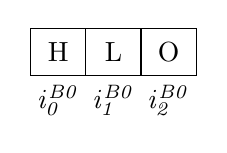
\begin{tikzpicture}
            \path
                node[letter, label=below:{\id{i}{B0}{0}}] {H}
                to ++(0:\widthletter) node[letter, label=below:{\id{i}{B0}{1}}] {L}
                to ++(0:\widthletter) node[letter, label=below:{\id{i}{B0}{2}}] {O};
        \end{tikzpicture}
        \caption{Elements with their corresponding identifiers}
        \label{fig:logootsplit-seq-as-letters}
    \end{subfigure}
    \begin{subfigure}{0.45\columnwidth}
        \centering
        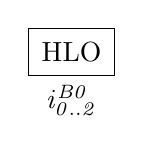
\begin{tikzpicture}
            \path
                node[block, label=below:{\id{i}{B0}{0..2}}] {HLO};
        \end{tikzpicture}
        \caption{Elements grouped into a block}
        \label{fig:logootsplit-seq-as-block}
    \end{subfigure}
    \caption{Representation of a LogootSplit sequence containing the elements "hlo"}
    \label{fig:logootsplit-seq}
\end{figure}

This feature allows to shift the cause of metadata growth from the number of elements to the number of blocks.
As blocks can contain an arbitrary number of elements, it enables to reduce significantly the memory overhead of the data structure.

\subsection{Limits}

As stated previously, the size of identifiers from a dense totally ordered set is variable.
When nodes insert new elements between two others with the same \emph{priority} value, LogootSplit has no other option than to increase the size of the resulting identifiers.
\autoref{fig:example-split} illustrates such cases.
In this example, since the node inserts a new element between contiguous identifiers, LogootSplit is not able to generate a fitting identifier of the same size. To comply with the intended order, LogootSplit generates the new identifier by appending to the predecessor's one a new tuple.

\begin{figure}
    \centering
    \begin{tikzpicture}
        \path
            node {\textbf{A}}
            to ++(0:\widthletter) node[block, label=below:{\id{i}{B0}{0..2}}] (HLO) {HLO}
            to ++(0:5 * \widthletter) node[letter, label=below:{\id{i}{B0}{0}}] (H) {H}
            to ++(0:\widthletter) node[letter, fill=mydarkorange, label=above:{\color{mydarkorange}\id{i}{B0}{0}\id{f}{A0}{0}}] {E}
            to ++(0:\widthletter) node[block, label=below:{\id{i}{B0}{1..2}}] {LO};

        \draw[->, thick] (HLO) -- node[below, align=center]{\emph{insert "e"}\\\emph{between}\\\emph{"h" and "l"}} (H);
    \end{tikzpicture}
    \caption{Insertion leading to longer identifiers}
    \label{fig:example-split}
\end{figure}

As a result, the size of identifiers tends to grow as the collaboration progresses.
This growth impacts negatively the performances of the data structure on several aspects.
Since identifiers attached to values become longer, the memory overhead of the data structure increases accordingly.
This also increases the bandwidth consumption as nodes have to broadcast identifiers to others.

Additionally, as the lifetime of the replicated sequence increases, the number of blocks composing it grows as well.
Indeed, several constraints on identifier generation prevent nodes from adding new elements to existing blocks.
For example, only the block's author can append or prepend elements to it.
These limitations cause the generation of new blocks.
Since no mechanism to merge blocks a posteriori is provided, the sequence ends up fragmented into many blocks.
The efficiency of the data structure decreases as each block introduces its own overhead.

In our benchmarks, we measure that these issues eventually lead to the content representing a fraction of the whole data structure's size, less than 1\%, as shown in \autoref{fig:overhead-size}. It is thus necessary to address them.

\begin{figure}
    \centering
    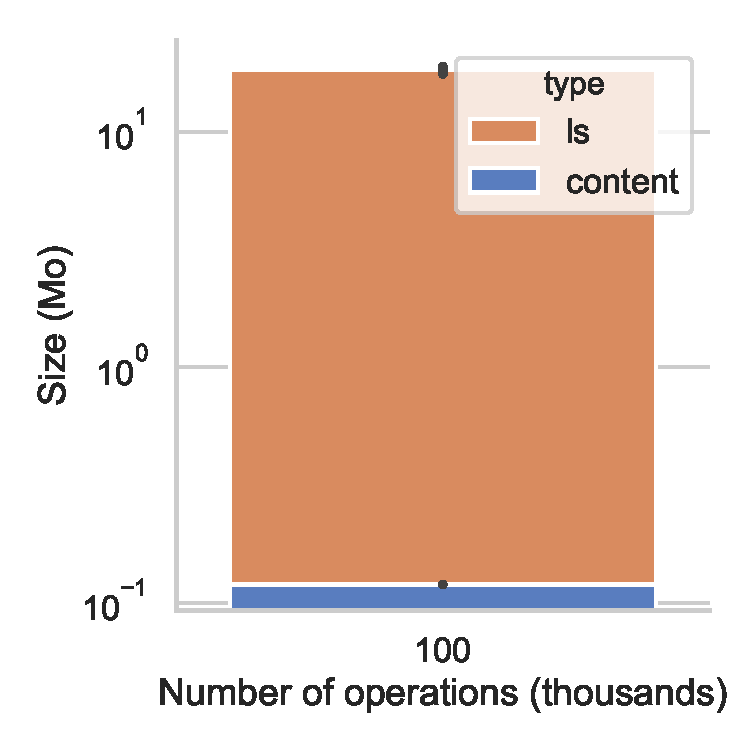
\includegraphics[width=0.55\columnwidth]{img/overhead-size.pdf}
    \caption{Footprint of the data structure}
    \label{fig:overhead-size}
\end{figure}

\subsection{Related works}

Over the years, several works were presented to reduce the growth of variable-size identifiers.
However, to the best of our knowledge, no works have been presented to decrease the number of blocks generated.

In \cite{letia:hal-01248270,zawirski:hal-01248197}, authors design for Treedoc \cite{5158449} a renaming mechanism to reassign shorter identifiers to elements.
Nodes rely on a consensus mechanism to trigger the renaming and a catch-up protocol to handle concurrent updates.
Since consensus algorithms are costly in large-scale distributed systems with churn, \citet{letia:hal-01248270} introduce a two-tier architecture.
Nodes are splitted between the \emph{core}, a set of stable and highly connected nodes, and the \emph{nebula} made of the remaining ones.
Every node can update the sequence but only members of the \emph{core} participate in the consensus leading to renaming.
However the \emph{core-nebula} approach is not suited to all kinds of applications.
In fully distributed systems, there is no central authority to provide the set of stable nodes acting as the \emph{core}.

In \cite{nedelec_2013_lseq,doi:10.1002/cpe.4108}, \citeauthor{nedelec_2013_lseq} introduce another approach to address the identifiers growth issue: LSEQ.
Its insight consists in using several strategies to select the \emph{priority} value of a new tuple.
These strategies prevent nodes from quickly saturating the space between two existing identifiers.
This approach enables to reduce the growth of identifiers.
And although the LSEQ approach has been designed for Logoot \cite{WeissICDCS09}, it can also be applied to LogootSplit.
However, its impact would be diminished as insertions into blocks result in new identifiers with increased sizes nonetheless.

\section{Proposed approach}
\label{sec:proposition}

We propose a new Sequence \ac{CRDT} belonging to the variable-size identifiers approach: \emph{RenamableLogootSplit} \cite{nicolas:hal-01932552}.

To address the limitations of LogootSplit, we embed in this data structure a renaming mechanism.
The purpose of this mechanism is to reassign shorter identifiers to elements and to regroup them into blocks to minimise the memory overhead of the whole sequence.

To avoid costly and blocking consensus algorithms, we instead adopt the \emph{optimistic replication} approach for this mechanism.
Nodes perform renaming without any coordination.
However, this operation is not intrinsically commutative with others.
If conflicts arise, we use \emph{operational transformations} to enable nodes to resolve them deterministically.
While transforming \emph{insert} and \emph{remove} operations against \emph{rename} one is straightforward, dealing with concurrent \emph{rename} operations is more tedious.
For the sake of simplicity and brevity, we focus in this paper only on the first case.
We leave the presentation and evaluation of required additional steps to handle concurrent \emph{rename} operations to a future work.

\subsection{System Model}

The system is composed of a dynamic set of nodes, as nodes join and leave dynamically the collaboration during its lifetime.
Nodes collaborate to build and maintain a sequence using RenamableLogootSplit.
Each node owns a copy of the sequence and edit it without any kind of coordination with others.

Nodes communicate through a \ac{P2P} network, which is unreliable.
Messages can be lost, re-ordered or delivered multiple times.
The network is also vulnerable to partitions, which split nodes into disjoined subgroups.
To overcome the failures of the network, nodes rely on a message-passing layer.
As RenamableLogootSplit is built on top of LogootSplit, it shares the same requirements for the operation delivery.
This layer is thus used to deliver messages to the application exactly-once.
The layer also ensures that \emph{remove} operations are delivered after corresponding \emph{insert} operations.
Nodes use an anti-entropy mechanism to synchronise in a pairwise manner, by detecting and re-exchanging lost operations.

\subsection{\emph{rename} operation}

\emph{RenamableLogootSplit} enables nodes to reduce the overhead of their replica by the means of a new operation: the \emph{rename} operation.
This operation reassigns arbitrary identifiers to elements.

\begin{figure}
    \begin{subfigure}{\columnwidth}
        \begin{tikzpicture}
            \path
                node {\textbf{A}}
                to ++(0:\widthletter) node[letter, label=below:{\id{i}{B0}{0}}] {H}
                to ++(0:\widthletter) node[letter, fill=mydarkorange, label=above:{\color{mydarkorange}\id{i}{B0}{0}\id{f}{A0}{0}}] {E}
                to ++(0:\widthletter) node[block, label=below:{\id{i}{B0}{1..2}}] (LO) {LO}
                to ++(0:4 * \widthletter) node[letter, fill=mydarkblue, label=below:{\color{mydarkblue}\id{i}{A1}{0}}] (H) {H};

            \draw[->, thick] (LO) -- node[below, align=center]{\emph{rename}} (H);
        \end{tikzpicture}
        \caption{Selecting the new identifier of the first element}
        \label{fig:renaming-first-id}
    \end{subfigure}
    \begin{subfigure}{\columnwidth}
        \begin{tikzpicture}
            \path
                node {\textbf{A}}
                to ++(0:\widthletter) node[letter, label=below:{\id{i}{B0}{0}}] {H}
                to ++(0:\widthletter) node[letter, fill=mydarkorange, label=above:{\color{mydarkorange}\id{i}{B0}{0}\id{f}{A0}{0}}] {E}
                to ++(0:\widthletter) node[block, label=below:{\id{i}{B0}{1..2}}] (LO) {LO}
                to ++(0:4 * \widthletter) node[letter, fill=mydarkblue, label=below:{\color{mydarkblue}\id{i}{A1}{0}}] (H) {H}
                to ++(0:\widthletter) node[letter, fill=mydarkblue, label=below:{\color{mydarkblue}\id{i}{A1}{1}}] {E};

            \draw[->, thick] (LO) -- node[below, align=center]{\emph{rename}} (H);
        \end{tikzpicture}
        \caption{Selecting the new identifier of the second one}
        \label{fig:renaming-second-id}
    \end{subfigure}
    \begin{subfigure}{\columnwidth}
        \begin{tikzpicture}
            \path
                node {\textbf{A}}
                to ++(0:\widthletter) node[letter, label=below:{\id{i}{B0}{0}}] {H}
                to ++(0:\widthletter) node[letter, fill=mydarkorange, label=above:{\color{mydarkorange}\id{i}{B0}{0}\id{f}{A0}{0}}] {E}
                to ++(0:\widthletter) node[block, label=below:{\id{i}{B0}{1..2}}] (LO) {LO}
                to ++(0:4 * \widthletter) node[block, fill=mydarkblue, label=below:{\color{mydarkblue}\id{i}{A1}{0..3}}] (HELO) {HELO};

            \draw[->, thick] (LO) -- node[below, align=center]{\emph{rename}} (HELO);
        \end{tikzpicture}
        \caption{Final state obtained}
        \label{fig:renaming-final-state}
    \end{subfigure}
    \caption{Renaming the sequence}
    \label{fig:renaming}
\end{figure}

Its behavior is illustrated in \autoref{fig:renaming} and can be described as follows:
\begin{enumerate*}
    \item It reuses the id of the first element of the sequence, but modified with the node's own id and sequence number (\autoref{fig:renaming-first-id})
    \item It generates contiguous identifiers for all following elements (\autoref{fig:renaming-second-id}).
\end{enumerate*}
As we assign contiguous identifiers to all elements of the sequence, we can eventually group them into one block as illustrated in \autoref{fig:renaming-final-state}.
It allows nodes to benefit the most from the block feature and to minimise the overhead of the resulting state.

In order for the system to eventually converge, other nodes have to rename their state identically.
To achieve this, the node issuing the \emph{rename} operation broadcasts its former state to others.
Using the former state, others compute the new identifier of each renamed identifier.
However, other nodes' states may contain concurrently inserted identifiers.
We will explain in \autoref{sec:dealing-with-concurrent-updates} how to rename them deterministically.

Broadcasting the \emph{rename} operation embedding the former state may be quite bandwidth consuming since the size of identifiers and the number of blocks are not bounded.
To partially address this issue, we propose a compression mechanism which sends only the necessary components to identify uniquely a block instead of whole identifiers.
This compression mechanism allows to reduce to a fixed amount per block the metadata to broadcast.

\subsection{Dealing with concurrent updates}

\label{sec:dealing-with-concurrent-updates}

As \emph{rename} operations can be issued without any kind of coordination, it is possible for other nodes to perform updates concurrently.
Since identifiers are modified by the \emph{renaming} mechanism, applying concurrent updates as they are would result in inconsistencies as illustrated in \autoref{fig:concurrent-insert-rename-inconsistent}.
It is thus necessary to handle concurrent operations to \emph{rename} operations in a particular manner.

\begin{figure}
    \begin{subfigure}{\columnwidth}
        \centering
        \begin{tikzpicture}
            \path
                node {\textbf{A}}
                to ++(0:2 * \widthletter) node[block, fill=mydarkblue, label=below:{\color{mydarkblue}\id{i}{A1}{0..3}}] (HELO) {HELO}
                to ++(0:4 * \widthletter) node[block, fill=mydarkblue, label=below:{\color{mydarkblue}\id{i}{A1}{0..3}}]  {HELO}
                to ++(0:\widthblock) node[cross, letter, fill=mylightorange, label=above:{\color{mylightorange}\id{i}{B0}{0}\id{m}{B1}{0}}] (right) {L};

            \path
                to ++(270:2) node {\textbf{B}}
                to ++(0:\widthletter) node[letter, label=below:{\id{i}{B0}{0}}] {H}
                to ++(0:\widthletter) node[letter, fill=mydarkorange, label=above:{\color{mydarkorange}\id{i}{B0}{0}\id{f}{A0}{0}}] {E}
                to ++(0:\widthletter) node[letter, fill=mylightorange, label=below:{\color{mylightorange}\id{i}{B0}{0}\id{m}{B1}{0}}] (left) {L}
                to ++(0:\widthletter) node[block, label=below:{\id{i}{B0}{1..2}}] {LO};

            \draw[dashed, ->, thick] (left.north) .. controls +(90:2 * \widthletter) and +(270:2 * \widthletter) .. node[below right, align=center]{\emph{insert}} (right.south);
        \end{tikzpicture}
        \caption{Concurrent update leading to inconsistency}
        \label{fig:concurrent-insert-rename-inconsistent}
    \end{subfigure}
    \begin{subfigure}{\columnwidth}
        \centering
        \begin{tikzpicture}
            \path
                node {\textbf{A}}
                to ++(0:2 * \widthletter) node[block, fill=mydarkblue, label=below:{\color{mydarkblue}\id{i}{A1}{0..3}}] (HELO) {HELO}
                to ++(0:4 * \widthletter) node[block, fill=mydarkblue, label=below:{\color{mydarkblue}\id{i}{A1}{0..1}}]  {HE}
                to ++(0:\widthblock) node[letter, fill=mylightblue, label=above:{\color{mylightblue!20!mydarkblue}\id{i}{A1}{1}\id{i}{B0}{0}\id{m}{B1}{0}}] (right) {L}
                to ++(0:\widthletter) node[block, fill=mydarkblue, label=below:{\color{mydarkblue}\id{i}{A1}{2..3}}]  {LO};


            \path
                to ++(270:2) node {\textbf{B}}
                to ++(0:\widthletter) node[letter, label=below:{\id{i}{B0}{0}}] {H}
                to ++(0:\widthletter) node[letter, fill=mydarkorange, label=above:{\color{mydarkorange}\id{i}{B0}{0}\id{f}{A0}{0}}] {E}
                to ++(0:\widthletter) node[letter, fill=mylightorange, label=below:{\color{mylightorange}\id{i}{B0}{0}\id{m}{B1}{0}}] (left) {L}
                to ++(0:\widthletter) node[block, label=below:{\id{i}{B0}{1..2}}] {LO};

            \draw[dashed, ->, thick] (left.north) .. controls +(90:2 * \widthletter) and +(270:2 * \widthletter) .. node[below right, align=center]{\emph{rename}\\ \emph{then insert}}(right.south);
        \end{tikzpicture}
        \caption{Fixed scenario}
        \label{fig:concurrent-insert-rename-fixed}
    \end{subfigure}
    \caption{Dealing with concurrent updates}
    \label{fig:concurrent-insert-rename}
\end{figure}

To detect them, we use an \emph{epoch-based} system.
We add an \emph{epoch} to the sequence as a property.
Each time a \emph{rename} operation is applied, the sequence progresses to a new epoch.
When nodes issue operation, they tag them with their current epoch.
Upon the reception of an operation, nodes compare their current epoch to the operation's one.
If they differ, nodes have to transform the operation before applying it.

To transform an operation, nodes use the algorithm described in \autoref{alg:renameId}.
This algorithm enables nodes to transform identifiers against the \emph{rename} operation.
The main idea of this algorithm is to use the predecessor of the given identifier to do so.
The algorithm consists mainly in
\begin{enumerate*}
    \item finding the predecessor of the given id in the former state
    \item computing its counterpart in the renamed state
    \item prepending it to the given id to generate the renamed id.
\end{enumerate*}
An example of its usage is illustrated in \autoref{fig:concurrent-insert-rename-fixed}.

Nodes use the same algorithm to rename identifiers they inserted concurrently when applying remote \emph{rename} operations.

Since nodes rely on the former state to transform concurrent operations to a \emph{rename} one, they have to store it.
Nodes need it until each of them can no longer issue concurrent operations to the corresponding \emph{rename} operation.
In other words, nodes can safely garbage collect the former state once the \emph{rename} operation became causally stable \cite{10.1007/978-3-662-43352-2_11}.
Meanwhile, nodes can offload it onto the disk as it is only required to handle concurrent operations.

\begin{algorithm}
    \caption{Rename identifier concurrently generated}
    \label{alg:renameId}
    \begin{algorithmic}
    \Function{renameId}{$\trm{id}, \trm{nId}, \trm{nSeq}, \trm{renamedBlocks}$}
        \State $\trm{length} \gets \trm{renamedBlocks.length}$
        \State $\trm{firstId} \gets \trm{idBegin}(\trm{renamedBlocks}[0])$
        \State $\trm{lastId} \gets \trm{idEnd}(\trm{renamedBlocks}[\trm{length} - 1])$\\

        \State $\trm{prior} \gets \trm{priority(firstId)}$
        \State $\trm{newFirstId} \gets \trm{new} \ \trm{Id}(\trm{prior}, \trm{nId}, \trm{nSeq}, 0)$
        \State $\trm{newLastId} \gets \trm{new} \ \trm{Id}(\trm{prior}, \trm{nId}, \trm{nSeq}, \trm{length - 1})$\\

        \If{$\trm{firstId} < \trm{id}$ \textbf{and} $\trm{id} < \trm{lastId}$}
            \State $\trm{pred} \gets \trm{findPredecessor}(\trm{id}, \trm{renamedBlocks})$
            \State $\trm{indexOfPred} \gets \trm{findIndex}(\trm{pred}, \trm{renamedBlocks})$
            \State $\trm{newPred} \gets \trm{new} \ \trm{Id}(\trm{prior}, \trm{nId}, \trm{nSeq}, \trm{indexOfPred})$
            \State \Return $\trm{concat}(\trm{newPredecessor}, \trm{id})$
        \ElsIf{$\trm{lastId} < \trm{id}$ \textbf{and} $\trm{id} < \trm{newLastId}$}
            \State \Return $\trm{concat}(\trm{newLastId}, \trm{id})$
        \ElsIf{$\trm{newFirstId} < \trm{id}$ \textbf{and} $\trm{id} < \trm{firstId}$}
            \State $\trm{predOfNewFirstId} \gets \trm{new} \ \trm{Id}(\trm{prior}, \trm{nId}, \trm{nSeq}, -1)$
            \State \Return $\trm{concat}(\trm{predOfNewFirstId}, \trm{id})$
        \Else
            \State \Return $\trm{id}$ \Comment Return the identifier unchanged as it does not interfere with the renaming
        \EndIf
    \EndFunction
    \end{algorithmic}
\end{algorithm}

\section{Evaluation}
\label{sec:evaluation}

\subsection{Simulations and benchmarks}

To validate the proposed renaming mechanism, we performed an experimental evaluation to measure its performances on several aspects:
\begin{enumerate*}
    \item the size of the data structure
    \item the integration time of \emph{insert} and \emph{remove} operations
    \item the integration time of the \emph{rename} operation.
\end{enumerate*}
In cases 1 and 2, we use LogootSplit as the baseline data structure to compare results.

% TODO: Reformuler cette phrase
Since we were not able to retrieve an existing dataset of traces of real-time collaborative editing sessions, we ran simulations to generate traces to evaluate our data structure.
The simulations depict the following scenario: several authors collaboratively write an article.
Initially, they prioritise adding content as everything remains to be done.
Thus they mainly insert elements into the document during this first phase.
A few \emph{remove} operations are still issued to simulate spelling mistakes.
Once the document reaches the critical length, collaborators switch to the second phase.
% TODO: Peut-être retravailler le "adding new content"
From this point, they stop adding new content and focus on revamping existing parts instead.
This is simulated by balancing the ratio between \emph{insert} and \emph{remove} operations.
Each author has to perform a given number of operations and the collaboration ends once all of them received all operations.
We take snapshots of the document at given steps of the collaboration to follow the evolution of the document.

We ran these simulations with the following experimental settings: we deployed 10 bots as separate Docker containers on a single workstation.
Each container corresponds to a single mono-threaded Node.js process (version 13.1.0) simulating an author.
The bots share and edit collaboratively the document using either LogootSplit or RenamableLogootSplit according to the session.
In both cases, each bot performs an \emph{insert} or a \emph{remove} operation locally every 200 $\pm$ 50ms.
During the first phase, the probabilities for each operation of being an \emph{insert} or a \emph{remove} are respectively of 80\% and 20\%.
% TODO: Glisser le terme "phase 2"
Once the document reaches 60k characters (around 15 pages), the probabilities are both set to 50\%.
Generated operations are broadcast to other nodes using a \ac{P2P} full mesh network.
After issuing an operation, there are 5\% of chances that the bot moves its cursor to another position in the document.
Each bot performs 15k operations.
Snapshots are taken every 10k operations overall.
Additionally, in the case of RenamableLogootSplit, one bot is arbitrarily designated as the master.
It performs \emph{rename} operations every 30k operations overall.

The code of the simulations is available at the following address: \url{https://github.com/coast-team/mute-bot-random/}.
This repository also contains the code corresponding to the benchmarks described in the next subsections as well as the results computed.

\begin{sloppypar}
Meanwhile, our implementation of LogootSplit and RenamableLogootSplit are available at \url{https://github.com/coast-team/mute-structs}.
Both implementations represent the sequence using an AVL Tree, a self-balancing binary search tree.
This data structure enables us to achieve \emph{insert} and \emph{remove} operations in logarithmic time.
\end{sloppypar}

\subsection{Results}

\paragraph{Memory overhead}

Using the snapshots generated, we compare the evolution of the size of the data structure in collaborative editing sessions.
\autoref{fig:evolution-document-size} presents the results.
On this plot, the blue line corresponds to the size of the content while the red one exhibits the growth of the LogootSplit data structure.

\begin{figure}
    \centering
    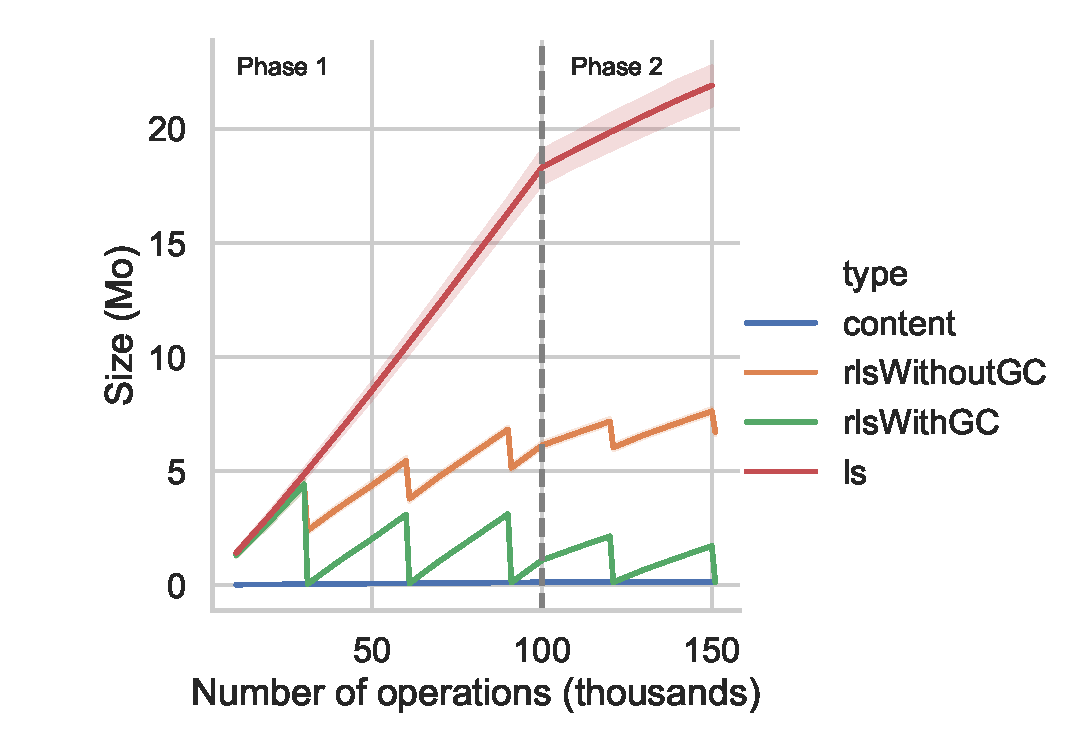
\includegraphics[width=0.9\columnwidth]{img/snapshots-sizes.pdf}
    \caption{Evolution of the size of the document}
    \label{fig:evolution-document-size}
\end{figure}

The green line illustrates the growth of the RenamableLogootSplit document in its best-case scenario.
In this scenario, \emph{rename} operations become stable as soon as they are issued.
Former states can then be garbage collected safely, maximising the benefits of the \emph{renaming} mechanism.
In this case, we observe that \emph{rename} operations reset the overhead of the data structure and eventually reduce by hundred times the document size compared to LogootSplit.

As for the orange line, it represents RenamableLogootSplit worst-case scenario.
Here, we assume that \emph{rename} operations never become causally stable and that nodes have to store former states forever.
However, obtained results show that RenamableLogootSplit outperforms LogootSplit and reduce by 66\% the size of the data structure, even in this case.
This outcome is explained by the fact that the AVL does not only store the content and blocks corresponding to the sequence.
Some metadata is actually added to the state to browse the sequence more efficiently when performing updates.
When a \emph{rename} operation is applied, nodes only keep the sequence of blocks from the former state as an array to be able to transform concurrent operations.
Other metadata is scrapped, which results in this memory gain.

\paragraph{Integration times of standard operations}

\begin{sloppypar}
We set up benchmarks to measure the impact of the renaming mechanism on the integration times of \emph{insert} and \emph{remove} operations.
The obtained results are presented in \autoref{fig:evolution-integration-time-insert-remove}.
\end{sloppypar}

\begin{figure}
    \begin{subfigure}{\columnwidth}
        \centering
        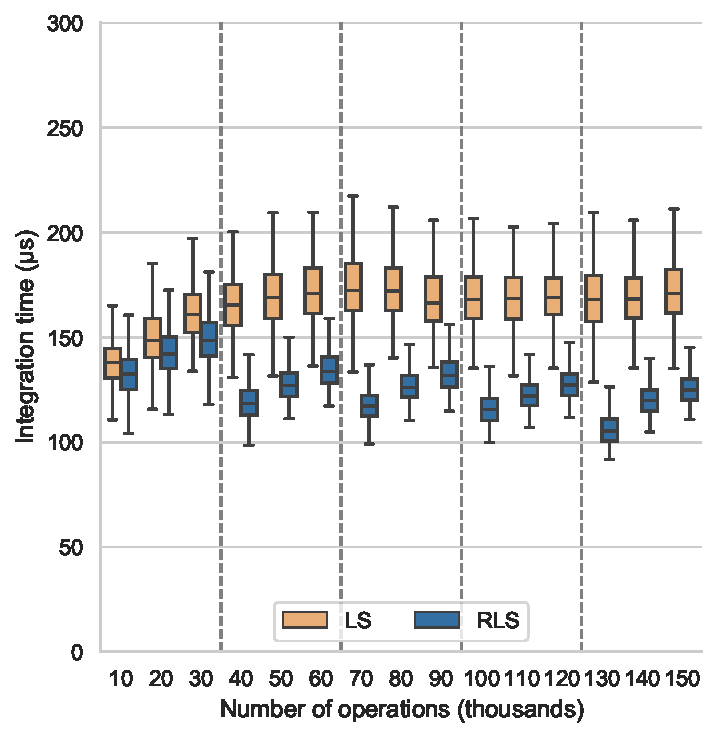
\includegraphics[width=0.9\columnwidth]{img/integration-time-boxplot-local-operations-without-outliers.pdf}
        \caption{Local operations}
        \label{fig:evolution-integration-time-local-insert-remove}
    \end{subfigure}
    \begin{subfigure}{\columnwidth}
        \centering
        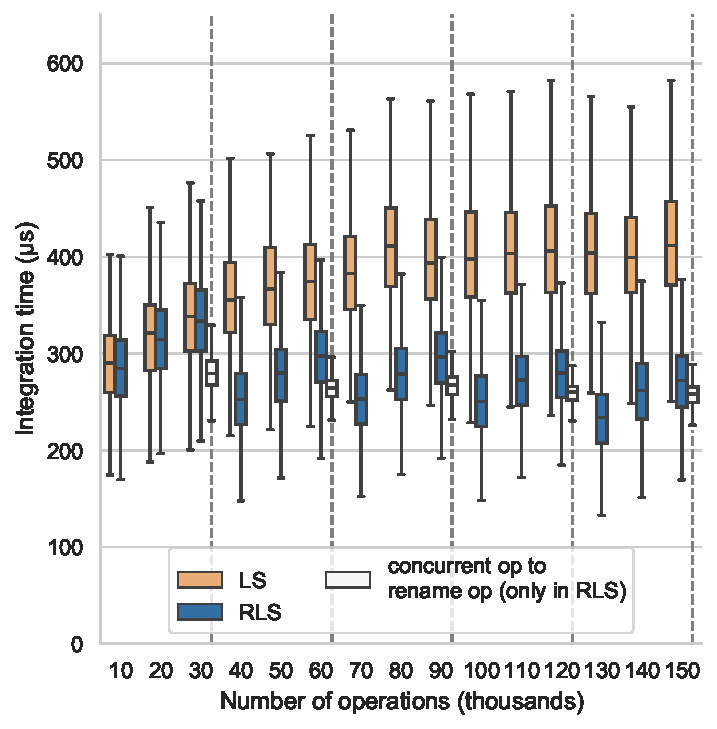
\includegraphics[width=0.9\columnwidth]{img/integration-time-boxplot-remote-operations-without-outliers.pdf}
        \caption{Remote operations}
        \label{fig:evolution-integration-time-remote-insert-remove}
    \end{subfigure}
    \caption{Evolution of the integration time of standard operations}
    \label{fig:evolution-integration-time-insert-remove}
\end{figure}

\autoref{fig:evolution-integration-time-local-insert-remove} displays the integration times of local operations while \autoref{fig:evolution-integration-time-remote-insert-remove} exhibits remote ones.
In both cases, the orange boxplots correspond to LogootSplit's integration times while blue ones to RenamableLogootSplit's ones.
The results show that the \emph{renaming} mechanism allows to reduce the integration times of future operations.

In \autoref{fig:evolution-integration-time-remote-insert-remove}, the green boxplots display the integration times of concurrent operations to a \emph{rename} one.
As illustrated in \autoref{sec:dealing-with-concurrent-updates}, these operations require to be transformed before being applied to the renamed state.
The results presented here show that this is actually faster than applying them directly on the former state.

\paragraph{Integration time of \emph{rename} operation}

Finally, we measured the integration time of the \emph{rename} operation according to the size of the document.
Results are displayed in \autoref{fig:evolution-integration-time-rename}.
In this figure, the blue line corresponds to the integration time of a \emph{local} rename operation while the orange one corresponds to the integration time of a remote one.

\begin{figure}
    \centering
    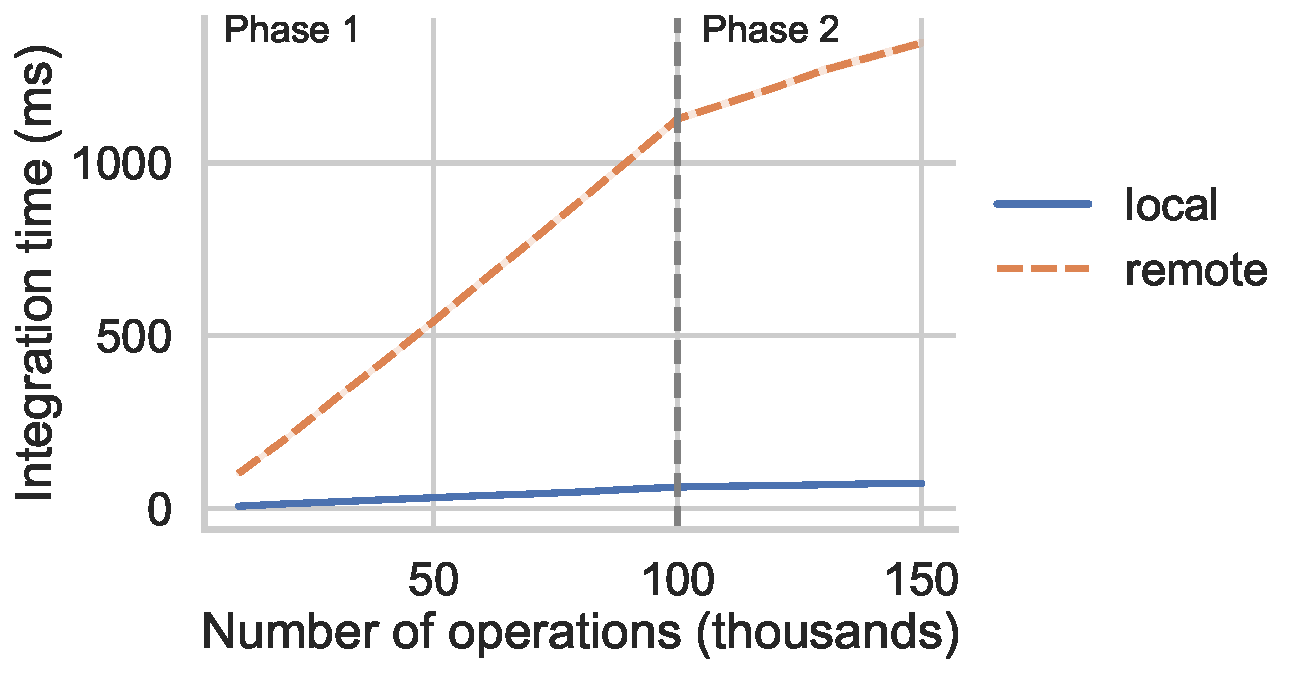
\includegraphics[width=0.9\columnwidth]{img/integration-time-rename.pdf}
    \caption{Evolution of the integration time of rename operations}
    \label{fig:evolution-integration-time-rename}
\end{figure}

The main result of this benchmark is that the unit of time used when applying \emph{rename} operations is in hundreds of milliseconds.
However other operations can not be integrated during the processing of \emph{rename} operations: remote operations won't be displayed to the user while local ones won't be propagated to others.
\emph{Rename} operations can thus be perceived as spikes of latency by users and degrade their experience if they are too long to process.
It is necessary to take this concern into account when designing the strategy used to trigger \emph{rename} operations to avoid such cases.

\section{Conclusions and future work}
\label{sec:conclusion}

In this paper, we introduced a novel Sequence \ac{CRDT} belonging to the variable-size identifiers approach: RenamableLogootSplit.
This new data structure embeds into its specification a renaming mechanism.
It enables nodes to reassign shorter identifiers to elements and group them into one block to minimise the metadata.

Obtained results experiments shown that RenamableLogootSplit reduces the overhead of the data structure by hundreds times compared to LogootSplit in the best-case scenario.
They also exhibited that it outperforms LogootSplit even in the worst-case one.
However, this comes at the price of an expensive but infrequent operation: the \emph{rename} operation.

As explained previously, \emph{rename} operations can be perceived by users as latency spikes if delayed for too long.
In order to prevent such user experience deterioration, it is necessary to set an upper-bound to their integration time.
User behaviour studies could be led in the context of real-time collaborative writing to identify this limit.

Finally, we designed RenamableLogootSplit with fully distributed systems in mind.
However, for the sake of simplicity, we presented it in this paper under the assumption that no concurrent \emph{rename} operations were issued.
This scenario is actually akin to systems in which nodes synchronise to trigger the renaming mechanism.
In a future work, we will introduce and evaluate the additional steps required to use RenamableLogootSplit in its original settings.

\bibliography{ref}

\end{document}
